% ============================================================
% Slide 5-8 (bản 45 phút) -- rút gọn từ part1.tex và part2.tex
% ============================================================

% --- Slide 5 (nguồn: part1.tex, "Tham số hoá hiệp phương sai") ---
\begin{frame}{Tham số hoá hiệp phương sai}
\begin{columns}
\begin{column}{0.55\textwidth}
\footnotesize
\begin{itemize}
    \item Không học trực tiếp $\Sigma$ để đảm bảo tính \textbf{positive semi-definite} khi tối ưu.
    \item Thay vào đó học scale $s \in \mathbb{R}^3$ và quaternion xoay $q \in \mathbb{R}^4$:
    \[
    \Sigma = R S S^T R^T
    \]
    với $S = \mathrm{diag}(s)$, $R = R(q)$.
\end{itemize}
\end{column}
\begin{column}{0.45\textwidth}
\centering

\includegraphics[width=0.78\linewidth]{ch1_scale_init.png}
\captionof{figure}{\footnotesize Khởi tạo scale từ khoảng cách lân cận}
\end{column}
\end{columns}
\end{frame}

% --- Slide 6 (nguồn: part1.tex, "Màu sắc qua Spherical Harmonics (SH)") ---
\begin{frame}{Màu sắc qua Spherical Harmonics (SH)}
\begin{columns}
\begin{column}{0.55\textwidth}
\footnotesize
\begin{itemize}
    \item Mỗi Gaussian không lưu 1 màu RGB cố định, mà lưu hệ số \textbf{SH}.
    \item Biểu diễn màu \textbf{phụ thuộc góc nhìn} (view-dependent), đặc tả hiệu ứng phản xạ/specular.
    \item Hệ số SH bậc 0 (DC) khởi tạo trực tiếp từ màu RGB quan sát được:
    \[
    f_{dc} = \mathrm{RGB2SH}(\text{color})
    \]
\end{itemize}
\end{column}
\begin{column}{0.45\textwidth}
\centering

\includegraphics[width=0.95\linewidth]{ch1_rgb2sh.png}
\captionof{figure}{\footnotesize Chuyển đổi RGB $\to$ hệ số SH bậc 0}
\end{column}
\end{columns}
\vspace{0.15cm}
\footnotesize
\textit{(Phần suy diễn toán học đầy đủ của SH được trình bày chi tiết trong bản đầy đủ, không đọc trong bản 45 phút.)}
\end{frame}

% --- Slide 7 (nguồn: part2.tex, "Tổng quan pipeline render") ---
\begin{frame}{Tổng quan pipeline render}
    \begin{itemize}
        \item World $\to$ Camera: biến đổi hệ toạ độ bằng view transform $(R, t)$
        \item Projection: chiếu các Gaussian 3D xuống mặt phẳng ảnh 2D
        \item Tiling + Sorting: xác định tile ảnh hưởng và sắp theo depth
        \item Alpha blending tuần tự $\to$ màu pixel cuối cùng
    \end{itemize}
    \vspace{0.3cm}
    \centering
    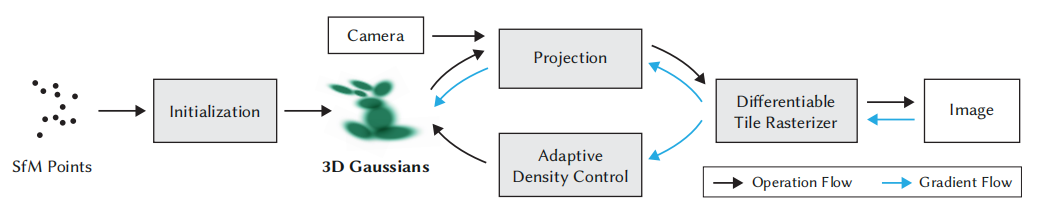
\includegraphics[width=0.95\linewidth]{pipe.png}
    \captionof{figure}{Pipeline render 3D Gaussian Splatting}
\end{frame}

% --- Slide 8 (nguồn: part2.tex, "Chiếu hiệp phương sai (EWA splatting)") ---
\begin{frame}{Chiếu hiệp phương sai (EWA splatting)}
    \begin{itemize}
        \item Phép chiếu phối cảnh phi tuyến $\to$ xấp xỉ tuyến tính cục bộ bằng Jacobian $J$ tại tâm Gaussian
        \item Hiệp phương sai 2D sau chiếu:
        \[
            \Sigma' = J\,W\,\Sigma\,W^{T}J^{T}
        \]
        trong đó $W$ là phần quay của view matrix
        \item Kỹ thuật này gọi là \textbf{Elliptical Weighted Average (EWA) splatting}
    \end{itemize}
    \vspace{0.2cm}
    \centering
    
\includegraphics[width=0.6\linewidth]{ch3_ewa_projection.png}
    \captionof{figure}{Chiếu hiệp phương sai theo EWA splatting}
\end{frame}
